\chapter{Encoded term format}
\label{encoded}

\go uses a special \emph{encoded term format} for a number of purposes -- such as when sending messages off-board and the format of compiled programs. This encoded term format is a binary format that is oriented for maximum efficiency in generating, parsing and storing.

In this appendix we describe this format, for those occasions where you may need explicit knowledge of the way the terms are handled and stored.

The encoded term format format is `self-parsing' and is able to represent symbols, numbers, arbitrary strings, program code, lists and tuples of  objects. Each of these types of structures have analogues in most programming languages: for example, the symbol type can be represented in Prolog as an atom, in \go as a symbol, and in C or Java as a string. The message format is even able to represent circular or graph structured values.

The self-parsing nature of the message format is important as it allows a great deal of flexibility: it is not necessary for the receiving agent of a message to be able to predict accurately the complete structure of a message prior to receiving it. 

The representation of values is network neutral, and quite efficient. For certain common cases, the low-level representation is optimized to minimize the length of the encoded message structure.

\section{Representation of values}
\label{encoded:representation}


The low-level structure of an encoded term consists of a sequence of 8bit bytes. Each object is preceded by a tag byte, followed by zero-or-more data value bytes. Some structures are nested -- such as lists and tuples -- in which case the elements of the nested structure follow the lead tag information.

The order of bytes in the encoded representation is well defined; and is independent of the natural byte order within words in computer memories -- no little-endian wars here. 

\subsection{Integer}
\label{encoded:integer}

The representation of integer values is a key aspect of the encoded term format -- since not are integer terms themselves represented using this format, but also many of the other kinds of terms -- such as the arity of tuples for example -- use the same basic representation.


An integer is represented as the byte \q{0x1\emph{k}} , where \emph{k} is in the range \q{0x1}\ldots{}\q{0xf}, followed by \emph{k} bytes defining the integer's value. The bytes making the value of the integer are in network -- that is most significant byte first -- order. The value is represented in standard 2's complement form.

For example, the integers \q{3} and \q{100,000} are represented by
the sequences:
\begin{alltt}
0x11 0x03
\end{alltt}
and
\begin{alltt}
0x13 0x01 0x86 0xa0
\end{alltt}
respectively.  Note that the value 0 is represented using the sequence \begin{alltt}
0x11 0x00
\end{alltt}

If the tag code is \q{0x10} then the length of the integer is itself expressed as an integer following the tag code, and the integer data itself follows the length. This allows arbitrary sized integers.

The following C program shows how an integer can be converted into the appropriate stream of bytes:

\begin{alltt}
unsigned char *EncodeInt(int tag,long long val,
                         unsigned char *buff)
\{
  int len=0;
  unsigned char bytes[16];
  unsigned long long v = val;

  if(v==0)              /* special case for 0 */
    bytes[len++]=0;
  else
    while(v>0)\{
      bytes[len++]=v&0xff;
      v >>= 8;
    \}

 *buff++=tag|len;       /* 0x1n \ldots{} */

  while(len-->0)
    *buff++=bytes[len];
  return buff;
\}
\end{alltt}

\subsubsection{Tagged length}
\label{encoded:tagged:length}

In many of the other encodings described below we require a numeric value to characterize them; for example, a string value has a length associated with it, as do constructor terms, and program code. We use the encoded integer format to represent the value; in general these numeric values have the form:
\begin{alltt}
0x\emph{k}\emph{n} 0xI\sub1 \ldots 0xI\subn
\end{alltt}
where \emph{k} is a \emph{key} that denotes the intended reading of the value (for example, strings use a key of \q{0x6}, constructors use a key of \q{0x9}. The integer value is encoded in the \emph{n} bytes \q{0xI\sub1}\ldots\q{0xI\subn} that follow the lead byte.

We will refer to this structure as a \emph{k}-\firstterm{tagged value} or a \emph{k}-tagged length where the tag \emph{k} is a number that characterizes the use of the value. Tagged values are typically followed by \emph{length} bytes or even \emph{length} complete encoded values.

%\begin{alltt}
%encodeInt(tg,val) => [bor(tg,len),..rev(L)] :-
%  val>=0,
%  L = encInt(val),
%  len = listlen(L).

%encInt(0,_) => [0].
%encInt(N,false)::N<256 => [N].
%encInt(N,true)::N<256 => [N,0].
%encInt(N,_) => [band(N,255),..encInt(bright(N,8),N>=0x80)].
%\end{alltt}

\subsection{Floating point encoding}
\label{encoded:float}

A floating point number is represented using the tag byte \q{0x2\emph{n}}, or \q{0x3\emph{n}} depending on whether the floating point number is positive or negative, followed by the exponent of the number -- in unbaissed form -- encoded in the same format as an integer and then \emph{n} bytes of mantissae.

The following C program shows how a floating point number can be
converted into the appropriate stream of bytes:

\begin{alltt}
/* Convert a double into a string buffer */
unsigned char *EncodeFlt(double f, unsigned char *buff)
\{
  unsigned char bytes[16], *bf = bytes;
 int i,exp,len,sign=0x20; /* positive float */

  if(f<0.0)\{
   sign = 0x30;         /* negative float */
    f = -f;
  \}

  f = frexp(f, &exp);

  for(len=0;f!=0.0;len++)\{
    double ip;
    f = modf(f*256,&ip);

    *bf++ = (int)ip;
  \}

 *buff++=sign|len;      /* the lead character of the number */
 buff = icmEncodeInt(exp,0x10,buff); /* the exponent */

  for(i=0;i<len;i++)
   *buff++=bytes[i];
  return buff;
\}
\end{alltt}

\subsection{Variables' encoding}
\label{encoded:variable}

There are two aspects of a variable's encoding: identifying the variable and linking different occurrences of the variable within a term. 

A variable occurrence is identified by a \q{0} tagged integer; i.e., a \q{0x0\emph{k}} byte, followed by \emph{k} bytes which encode a \emph{variable number} in the same format as an integer.

The scope rules for variables are not defined by the encoding; although a `decoding engine' is required to differentiate variables within a single encoded term. If it is required to properly scope variable occurrences within an encoded term then one should use the variable encoding in conjunction with the tag and reference encoding.

For example, to encode an expression such as:
\begin{alltt}
(x,x)
\end{alltt}
one could use a tag/variable (see Section~\vref{encoded:graph}) combination for the first occurrence of \q{x} and a reference for the subsequence occurrences. This would result in the sequence:
\begin{alltt}
0x91 0x01 0xa1 0x00 0x01 0x00 0xb1 0x00
\end{alltt}

\subsection{Symbol encoding}
\label{encoded:symbol}

A symbol is represented by a \q{4}-tagged length, followed by the characters of the symbol itself -- encoded in UTF-8.

For example, the symbol \q{'apple'} is represented by the sequence:

\begin{alltt}
0x41 0x05 0x61 0x70 0x70 0x6c 0x6e
\end{alltt}

\subsection{Character encoding}
\label{encoded:char}

A character literal is represented by a leading \q{0x4\emph{k}} byte, where \emph{k} is a number in the range \q{0x1}\ldots\q{0xf} followed by \emph{k} bytes which encode the character as a Unicode value. Note that the character is NOT encoded in UTF-8, its actual Unicode code value is directly encoded as an integer.

\subsection{String encoding}
\label{encoded:string}

A string or uninterpreted data block contains bytes that are not interpreted as having an internal structure. Their type is analogous to a string in Java or \go.

A string is represented with a leading \q{0x6}-tagged length, followed by the characters of the string -- encoded in UTF-8.

For example, the string: \q{"apple"} is encoded as the byte sequence:

\begin{alltt}
0x61 0x05 0x61 0x70 0x70 0x6c 0x6e
\end{alltt}
Note that \go is Unicode based, however, the sequence of bytes that form the string is encoded in UTF-8

\subsection{Program code}
\label{encoded:code}

The encoding for program code has two layers -- in the first layer a block of bytes is signalled as a code block. The encoding supports code blocks for different languages, not only \go.

A program code is necessarily quite platform specific. In our representation of program codes, we assume that there is an internal method for verifying that a piece of program code is of the correct structure. From the point of view of the encoded term format, program codes are encoded in a similar manner to uninterpreted strings or uninterpreted data blocks.

A program code is represented with a leading \q{0x7\emph{k}} byte, where \emph{k} is a number in the range \q{0x0}\ldots{}\q{0xf} followed by a length number \emph{N} -- itself encoded in \emph{k} bytes -- followed by \emph{N} bytes of data.


\subsection{List encoding}
\label{encoded:list}

A list is a sequence of values, intended to be held either in a Prolog, LISP or \go style list, or as an array of values in languages such as C, or Java.

Lists come in two `sizes': the empty list and the non-empty list. An empty list is represented by the \q{0x80} byte -- with no data following it -- and a non-empty list consists of the \q{0x81} byte, followed by the encoding of the head of the list, followed by the encoding of the tail of the list.

For example, the list of integer:
\begin{alltt}
[1,2,3]
\end{alltt}
is encoded using the sequence:
\begin{alltt}
0x81 0x11 0x01                              -- [1,
     0x81 0x11 0x02                         --  2,
          0x81 0x11 0x03                    --  3
               0x80                         --  ]
\end{alltt}

\subsection{Structure encoding}
\label{encoded:structure}

A structure includes tuples and constructor terms. A structure is encoded using a \q{9}-tagged length, followed by length encoded terms. The first element in the sequence should be a symbol which is either the constructor function's name or the symbol \q{()} to indicate a tuple.


For example, the \go tuple
\begin{alltt}
('fred', 23, [])
\end{alltt}

would be represented using the sequence:
\begin{alltt}
0x91 0x04                       -- A 4-element structure
  0x41 0x02 0x28 0x29           -- Its a tuple
  0x41 0x04 0x66 0x72 0x65 0x64 -- 'fred'
  0x11 0x17                     -- 23
  0x80                          -- []
\end{alltt}


\section{Objects}
\label{encoded:objects}

An object is represented as a sequence of all the element names and values in the object. An object is encoded using a \q{f}-tagged length, where the length is the number of attributes in the set. Each element is encoded as two values in sequence: the method name -- encoded as a symbol -- and the value.

An important constraint is that the \emph{order} of elements in an object is important: they must be in ascending order of method names -- more particularly in ascending UNICODE encoding order. Failure to meet this requirement may result in elements of objects that are not processable by the \go engine.

For example, an object with elements:
\begin{alltt}
\{. \$class/[person[]], \$obj/'person234', name/'fred', age/23 .\}
\end{alltt}
would be represented using the sequence:
\begin{alltt}
0xf1 0x04                       -- four elements
  0x41 0x06 0x24 0x63 0x6e 0x61 0x73 0x73 -- \$class
  0x81                          -- [
    0x91 0x00 0x06 0x70 0x65 0x72 0x73 0x6f 0x6d -- person[]
    0x80                        -- ]
  0x41 0x04 0x24 0x6f 0x62 0x6a -- \$obj
  0x41 0x09 0x70 0x65 ...  0x6e 0x32 0x33 0x34 -- person234
  0x41 0x03 0x61 0x67 0x65      -- age 
  0x11 0x17                     -- age value
  0x41 0x04 0x6e 0x61 0x6d 0x65 -- name
  0x41 0x04 0x66 0x72 0x65 0x64 -- 'fred'
\end{alltt}

\section{Circular structure and graph structures}
\label{encoded:graph}

Some structures must be represented using some kind of circular or graphical structure combination of lists and tuples. An important example of this is a program \emph{closure}. The term encoding permits this through the use of tags and references. A tag is a marker that identifies a particular structure -- giving it a kind of label. A reference is a reference to a structure that is marked elsewhere in the message: the value denoted by a reference is the value marked by the corresponding tag.

With this, we can embed circular and arbitrary graphical structures in messages and reproduce their structure when the message is decoded.

A tag is represented as the byte \q{0xa\emph{n}} -- where \emph{n} is a number in the range \q{0x0}\ldots{}\q{0xf} -- followed by \emph{n} bytes which encode a tag number \emph{N}; followed by the encoding of the tagged structure itself.

A reference is represented using the byte \q{0xB\emph{n}} -- where \emph{n} is a number in the range \q{0x0}\ldots{}\q{0xf} -- followed by \emph{n} bytes which encode a tag number \emph{N}. The `value' of the encoded structure is determined by the previously decoded tagged object for the same \emph{N}.

For example, the following circular structure:

\begin{alltt}
L0: (foo, 23, R0)
\end{alltt}

where \q{R0} is a reference to the complete tuple, can be encoded using:
\begin{alltt}
0xA1 0x00                                      -- L0:
     0x91 0x04 0x41 0x28 0x29                  -- ( tuple
               0x41 0x03 0x66 0x6f 0x6f        -- foo
               0x11 0x17                       -- 23
               0xB1 0x00                       -- R0
\end{alltt}

\subsection{Shorthand references}
\label{encoded:short}

A shorthand reference allows significant message compression by avoiding repetition of elements of the message. The basic form of a shorthand reference consists of a definition followed by a structure which may (or may not) embed a reference to the definiens.

A shorthard definition is encoded using the lead byte \q{0xc\emph{n}} -- where \emph{n} is a number in the range \q{0x0}\ldots{}\q{0xf} -- followed by a number \emph{N} which is the \emph{key}, followed by an encoded term -- which is the definiens -- followed by a second encoded term -- which is the `value' of the entire sequence.

Note that \go itself does not currently \emph{generate} any shorthand references but it is able to \emph{decode} them correctly.


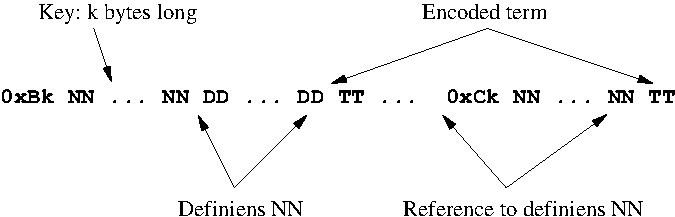
\includegraphics{shorthand}

For example, the structure

\begin{alltt}
('foo', ('bar', 'foo'), 'foo')
\end{alltt}

would normally be represented using the sequence:

\begin{alltt}
0x91 0x04 0x41 0x02 0x28 0x29             -- ( tuple
     0x41 0x03 0x66 0x6f 0x6f             -- foo
     0x91 0x03 0x41 0x02 0x28 0x29        -- (tuple
               0x41 0x03 0x62 0x61 0x72   --  bar
               0x41 0x03 0x66 0x6f 0x6f   -- foo )
     0x41 0x03 0x66 0x6f 0x6f             -- foo)
\end{alltt}

There are three references to the symbol \q{foo}. Normally, each reference would result in the symbol's name being represented in full; however, using a shorthand reference we can instead represent the structure using:

\begin{alltt}
0xc1 0x00 0x41 0x02 0x28 0x29             -- L0=()
0xc1 0x01 0x41 0x03 0x66 0x6f 0x6f        -- L1=foo
     0x91 0x04 0xB1 0x00                  -- ( ref L0
          0xB1 0x01                       -- R1:foo
          0x91 0x03 0xb1 0x00             -- ( ref L0
                    0x41 0x03 0x62 0x61 0x72   --  bar
                    0xb1 0x01              -- R1:foo )
      0xB1 0x01                            -- R1:foo)

\end{alltt}
which is both a little shorter than the original but also more efficient to decode.

Note that references to the shorthand object are made using the same encoded sequence as references to values in a circular structure. 

The \emph{scope} of a shorthand reference is the single encoded term that immediately follows the definition. It is possible for a sub-structure to also contain shorthand references; furthermore, it is possible to re-use a given shorthand reference code. In this latter case the inner definition of the shorthand reference overrides the outer definition of the shorthand reference.

\section{Representing types}
\label{encoded:types}

\go programs occasionally communicate values with embedded type expressions within them; this is particularly true for those type that have \emph{existential type variables} -- values of such types must have a type expression included within them that represents the value of the existential type variable for that expression.

For example, an \q{any}-type expression such as:
\begin{alltt}
??(34)
\end{alltt}
has a run-time representation analogous to:
\begin{alltt}
??(34,number)
\end{alltt}

Type expressions are represented using the same basic mechanisms as for representing other terms. However, we use additional internal `cues' to distinguish type terms from other terms. 

Type terms come in two basic forms -- particular type symbols and particular type constructors. 

\subsection{Type symbols}
\label{encoded:type:symbol}

All non-polymorphic types are represented using a symbol. The encoding for a type symbol is the same as for a regular program symbol; except that the symbol's first character is always \q{\hash}. For example, the run-time symbol used to represent the \q{number} type is \q{'\#number'}. Thus the representation of the expression \q{??(34)} is:

\begin{alltt}
0x91 0x03
     0x41 0x02 `? `?               -- ??
     0x11 0x32                     -- 34
     0x41 0x07 `# `n `u `m `b `e `r -- #number
\end{alltt}

\subsection{Type constructors}
\label{encoded:type:constructor}

Type constructors are represented in a similar way to regular constructors, except that the constructor's function symbol's first character is always a \q{\hash}. For example, the symbol used to denote a function type is \q{\hash{}=>}, and the representation of the type expression:
\begin{alltt}
(number,number) => number
\end{alltt}
is
\begin{alltt}
0x91 0x03 0x41 0x03 `# `= `>
     0x91 0x03 0x41 0x03 `# `( `)
               0x41 0x07 `# `n `u `m `b `e `r
               0x41 0x07 `# `n `u `m `b `e `r
     0x41 0x07 `# `n `u `m `b `e `r
\end{alltt}

The standard type constructors are:
\begin{description}
\item[\q{()}] Tuple types use the \q{\hash()} type constructor symbol.
\item[\q{\classtype}] Function types use the \q{\hash\classtype} type constructor symbol.
\item[\q{=>}] Function types use the \q{\hash=>} type constructor symbol.
\item[\q{\{\}}] Predicate types use the \q{\hash\{\}} type constructor symbol.
\item[\q{*}] Action types use the \q{\hash*} type constructor symbol.
\item[\q{-->}] Grammar types use the \q{\hash-->} type constructor symbol.
\item[\q{-}] Quantified types use the \q{\hash-} type constructor symbol.
\item[\q{[]}] List types use the \q{\hash[]} type constructor symbol.
\end{description}

User defined polymorphic (and object) types have a type constructor symbol of the form:
\begin{alltt}
#\emph{name}
\end{alltt}
A type expression such as
\begin{alltt}
tree(symbol)
\end{alltt}
would be represented as:
\begin{alltt}
0x91 0x02 0x41 0x05 `# `t `r `e `e 
          0x41 0x07 `# `n `u `m `b `e `r
\end{alltt}

\subsection{Variables in types}
\label{encoded:types:variable}

A type variable occurring in a type expression is representing using the same mechanisms as regular variables. Note, however, that most type variables occuring in a type expression are expected to be \emph{bound} -- i.e., scoped within an explicit universal type quantifier expression.


\section{Encoded terms in files}
\label{encoded:terms}

A complete encoded term -- as a separate unit on a file stream for example -- is encoded as a string (see section~\vref{encoded:string}). I.e., there is an outer wrapper to encoded terms that gives the length of the entire encoded expression. The characters of the string are derived from encoding the term itself. This has the advantage that encoded terms are always `self-parsing' when presented on actual file streams.

Furthermore, a \emph{file} that contains an encoded term may be optionally prefixed by a shell escape, such as
\begin{alltt}
#!/opt/go/bin/go
\end{alltt}
The purpose of this is to support the Unix shell script convention where a `data file' may be interpreted as a shell script. This permits, for example, a compiled \go program to be executed as though it were a binary or regular script.

